
%%---------------------------------------------------------------------
%	Preamble
%	AMS gruppe 12
%	AMS F18
%---------------------------------------------------------------------
\documentclass[12pt,fleqn,a4paper]{article}
\usepackage[utf8]{inputenc}
\usepackage[danish]{babel}
\usepackage[top=2.5cm, left=2cm, right=2cm, bottom=2.5cm]{geometry}
\usepackage{graphicx}
\usepackage[bottom]{footmisc}
\usepackage{framed}
\usepackage{caption}
\usepackage{float}
\usepackage{mdframed}
\usepackage{listings}
\usepackage{color}
\usepackage[T1]{fontenc}
\usepackage{amsmath,amsfonts,amsthm} % Math packages
\usepackage{array}
\usepackage{wrapfig}
\usepackage{multirow}
\usepackage{tabu}
\usepackage{longtable}
\usepackage{lastpage}
\usepackage{fancyhdr}
\usepackage[compact]{titlesec}
\usepackage[table,xcdraw]{xcolor}
\usepackage{arydshln}
\usepackage[isbn,issn,url]{dk-bib}
\usepackage[toc,page]{appendix}
\usepackage{url}
\def\UrlBreaks{\do\/\do-}

\definecolor{mygreen}{RGB}{28,172,0} % color values Red, Green, Blue
\definecolor{mylilas}{RGB}{170,55,241}
\renewcommand{\lstlistingname}{Kodeudsnit}
\tabulinesep=3mm

\setcounter{secnumdepth}{2}
\setcounter{tocdepth}{2}

\setlength{\parindent}{0mm} %intet indryk
\setlength{\parskip}{3mm} 	%linjeskift v. afsnit

% Ændring af enumerize og itemize 
\usepackage{enumitem} % @http://ctan.org/pkg/enumitem
\setlist[itemize]{topsep=0pt, itemsep=0.5pt}
\setlist[enumerate]{topsep=0pt, itemsep=0.5pt}

%afstand omkring sections
\titlespacing{\section}{0pt}{5mm}{0pt}
\titlespacing{\subsection}{0pt}{2mm}{0pt}
\titlespacing{\subsubsection}{0pt}{2mm}{0pt}

\usepackage{arydshln}
%aryd
\setlength\dashlinedash{3pt}
\setlength\dashlinegap{4pt}

\lstset{language=C++,
	breaklines=true,
	keywordstyle=\color{blue},
	stringstyle=\color{red},
	commentstyle=\color{mygreen},
	morecomment=[l][\color{magenta}]{\#}
}

%header & footer
\makeatletter
\pagestyle{fancy}
\fancypagestyle{plain}{}
\renewcommand{\chaptermark}[1]{\markboth{#1}{}}
\setlength{\headheight}{35pt}
\fancyfoot{} % clear all fields
\fancyfoot[R]{Side \thepage\ af \pageref{LastPage}}
\fancyhead{} % clear all fields
\fancyhead[L]{
\includegraphics[clip, trim = 0 0 240pt 0, height=30pt]{Figur/IHA_AU_logo.png}}
\fancyhead[R]{Forår 2018}
\fancyhead[C]{Anvendte Microcontroller Systemer}
\renewcommand{\headrulewidth}{0pt}

\def\thickhrulefill{\leavevmode \leaders \hrule height 1.2ex \hfill \kern \z@}
\def\@makechapterhead#1{
  \vspace*{10\p@}%
  {\parindent \z@ \centering \reset@font
        \thickhrulefill\quad 
        \scshape\bfseries\textit{\@chapapp{}  \thechapter}  
        \quad \thickhrulefill
        \par\nobreak
        \vspace*{10\p@}%
        \interlinepenalty\@M
        \hrule
        \vspace*{10\p@}%
        \Huge \bfseries #1 \par\nobreak
        \par
        \vspace*{10\p@}%
        \hrule
        \vskip 40\p@
  }}

\usepackage{tcolorbox}
\definecolor{mycolor}{rgb}{0.122, 0.435, 0.698}% Rule colour
\makeatletter
\newcommand{\mybox}[1]{%
	\setbox0=\hbox{#1}%
	\setlength{\@tempdima}{\dimexpr\wd0+13pt}%
	\begin{tcolorbox}[colframe=mycolor,boxrule=0.5pt,arc=4pt,
		left=6pt,right=6pt,top=6pt,bottom=6pt,boxsep=0pt]
		#1
	\end{tcolorbox}
}
\makeatother

\graphicspath{ {Figur/} }


%Se Kodeudsnit \ref{lstlisting:generel_kode}

%\captionof{lstlisting}{Generelle egenskaber for koden til fremstilling af diverse figure i matlab} 
%\label{lstlisting:generel_kode}
%\vspace{5mm} %5mm vertical space
%
%\subsection{Kode til lyd i forhold til tiden}
%\begin{framed}
%\begin{center}
%\begin{lstlisting}
%figure('name','trafikstoejen i fuld laengde'); clf
%subplot(211);
%plot(t,s_sound_left)
%xlabel('Tid (sek)')
%ylabel('Signalstyrke')
%title('Trafikstoej set i forhold til tiden')
%grid on
%hold on
%\end{lstlisting}
%\end{center}
%\end{framed}





%\begin{document}
%	KRAVSPECIFIKATION

\chapter{Krav}
\section {Systemoversigt}

Systemet består af en PC, der indeholder det meste af systemets kontrollogik.

PC'en har:
\begin{itemize}
\item Tilsluttet et kamera, der bruges til at analysere brugerens øjenbevægelser. 
\item En trådløs forbindelse til robotten, der bruges til at sende og modtage data mellem enhederne, bl.a. til at modtage et videofeed.
\item Et GUI, hvorpå brugeren kan se videofeedet fra robotten, samt styre systemet via et kamera-input.\newline
\end{itemize} 

Systemet består derudover af en robot som kontrolleres via PC'en.

Robotten har:
\begin{itemize}
\item Motorer og hjul, der gør, at den kan køre, samt dreje om egen akse.
\item En kontrolenhed, der kommunikerer med PC'en. 
Kontrolenheden kontrollerer en motorstyringsenhed, der kontrollerer og regulerer motorerne.
\item Et kamera, der filmer i køreretningen. Videofeedet bliver streamet til PC'en gennem kontrolenheden.\newline
\end{itemize}

På figur \ref{fig:dele_i_system} og \ref{fig:RobotIndhold} ses en koncepttegning af systemet og en illustration af robottens indhold.

\begin{figure} [H]
\centering
	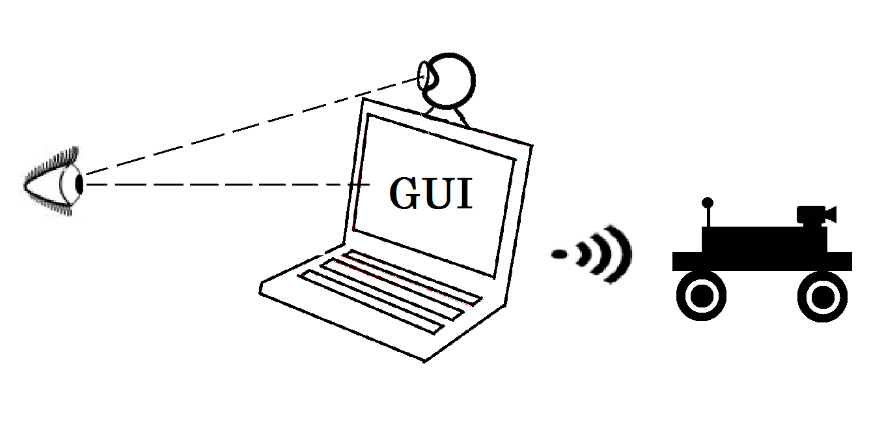
\includegraphics[width=0.7 \textwidth]{dele_i_system.png}
	\captionof{figure}{Illustration af de forskellige dele systemet består af}
	\label{fig:dele_i_system}
\end{figure}


\begin{figure} [H]
\centering
	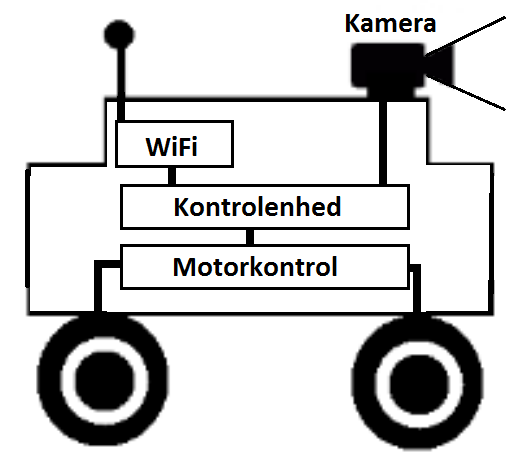
\includegraphics[width=0.3 \textwidth]{RobotIndhold.png}
	\captionof{figure}{Illustration af robottens indhold}
	\label{fig:RobotIndhold}
\end{figure}


\section{MoSCoW}
I dette afsnit findes en analyse ud fra MoSCoW analyse \cite{moscow}. 

I prototypen er implementeret alle punkter fra "Skal" og "Bør".

Skal/Must:
\begin{enumerate}
	\item Systemet \textbf{skal} kunne betjenes med øjnene
	\item Systemet \textbf{skal} interagere med brugeren vha. et GUI
	\item Systemet \textbf{skal} indeholde en PC-applikation
	\item PC-applikationen og robotten \textbf{skal} kommunikere trådløst
	\item Robotten \textbf{skal} sende et videofeed til PC'en
	\item Robotten \textbf{skal} kunne dreje om egen akse
\end{enumerate}
Bør/Should:
\begin{enumerate}
	\item Robottens videofeed \textbf{bør} vises på GUI i realtid
	\item Systemet \textbf{bør} have en standardiseret port til udvidelsesmoduler
\end{enumerate}
Kunne/Could:
\begin{enumerate}
	\item Robotten \textbf{kunne} have påmonteret lys
	\item Robottens lys \textbf{kunne} automatisk aktiveres/deaktiveres ift. lysintensitet
	\item Robotten \textbf{kunne} tilslutte sig en ladestation
	\item Systemet \textbf{kunne} overvåge spændingsniveauet på robottens batteri
	\item Systemet \textbf{kunne} overvåge signalstyrken mellem PC og robot
	
\end{enumerate}
Vil ikke/Won’t:
\begin{enumerate}
	\item Systemet \textbf{vil ikke} kunne tage højde for at brugeren bruger briller el.l.
	\item Systemet \textbf{vil ikke} kunne advare brugeren, hvis Robotten kommer indenfor en given minimumsafstand til et objekt
	 \newline
\end{enumerate}


\section{Grafisk brugerflade}
I dette afsnit beskrives systemets grafiske brugerflade. Denne kan ses på figur \ref{fig:GUI_drive_and_hold} og figur \ref{fig:GUI_hold_and_menu}.
GUI'et består af to skærme, en køreskærm og en menuskærm. 

\begin{center}
	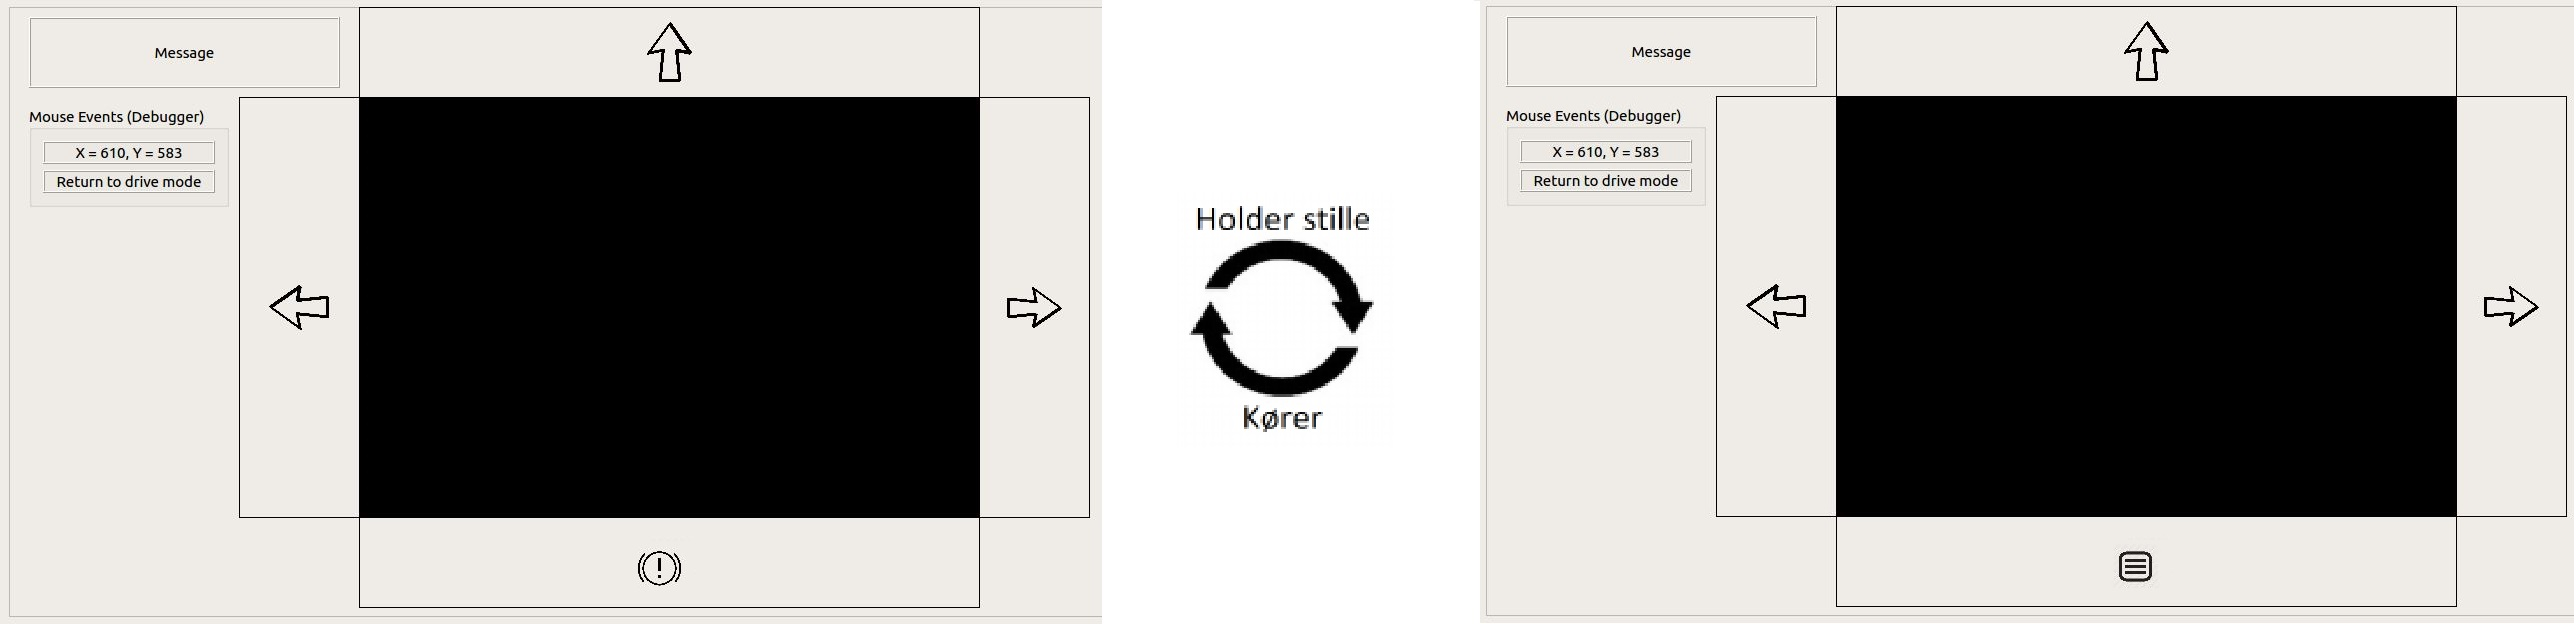
\includegraphics[width=0.9 \textwidth]{MenuIconToBrakeIcon.JPG}
	\captionof{figure}{Viser køreskærmen, hvor der skiftes mellem bremse- og menuikon}
	\label{fig:GUI_drive_and_hold}
\end{center}

\begin{center}
	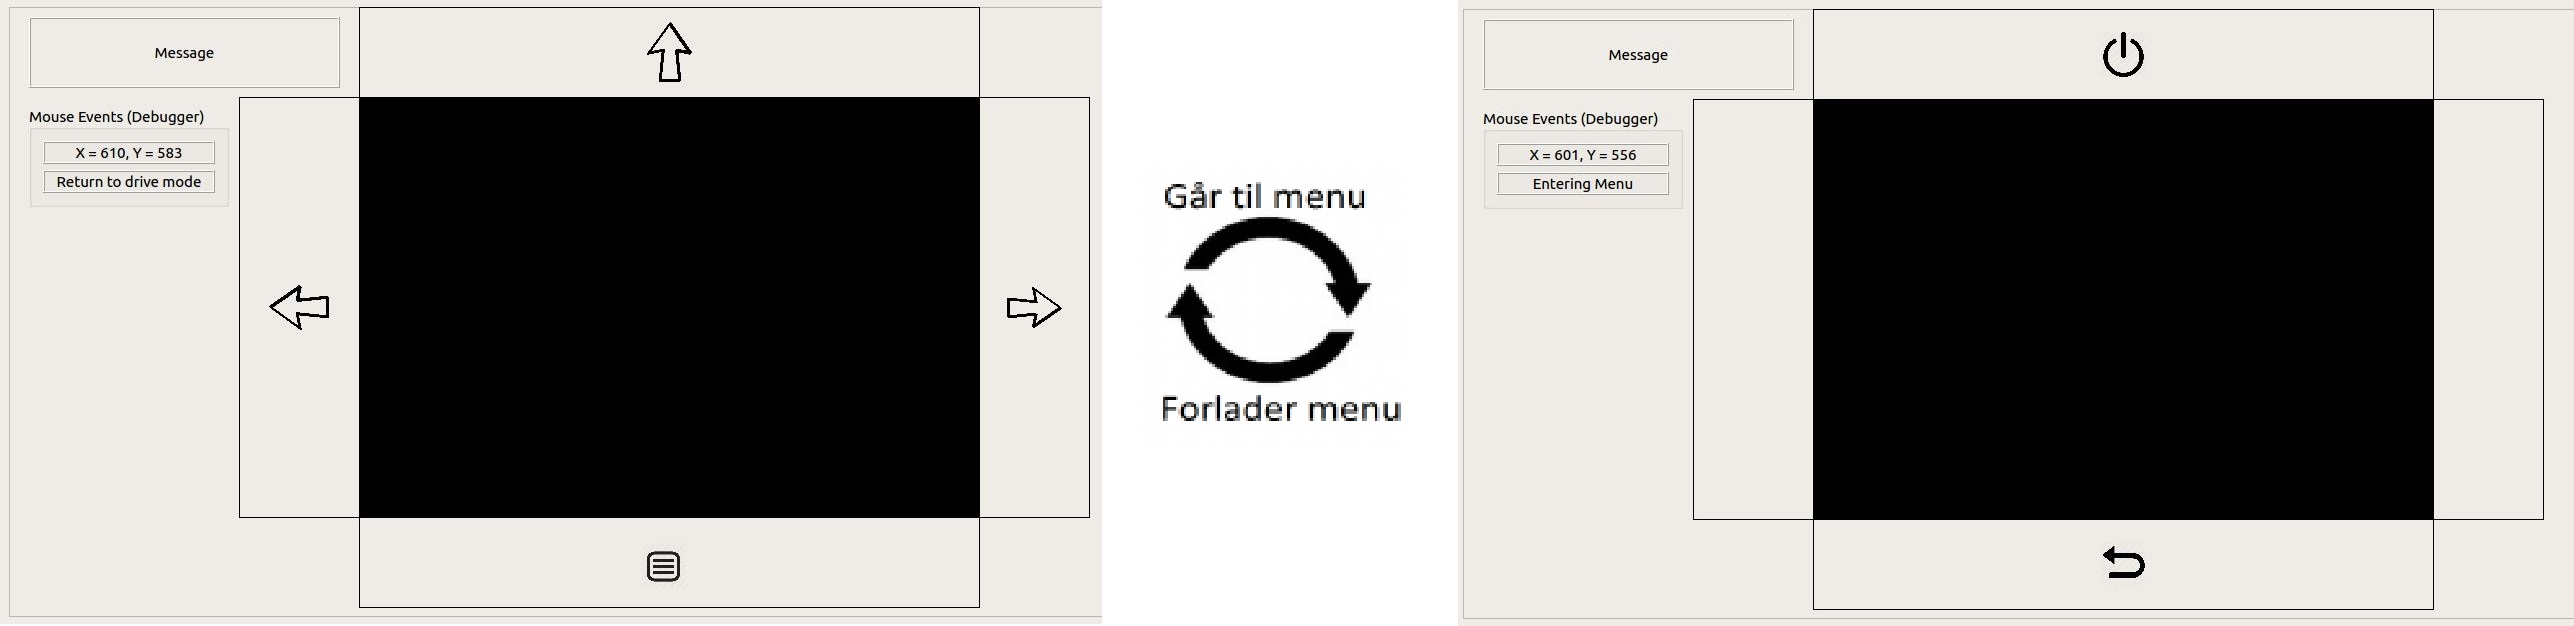
\includegraphics[width=0.9 \textwidth]{DriveToMenuScreen.JPG}
	\captionof{figure}{Viser hvordan der skiftes imellem køre- og menuskærmen}
	\label{fig:GUI_hold_and_menu}
\end{center}


\begin{itemize}
	\item \textit{Køreskærmen} giver brugeren mulighed for at styre robotten. Bremse- og menuikonet i bunden af skærmen vises når robotten er henholdsvis i bevægelse eller stoppet.
	\item \textit{Menuskærmen} vises, når brugeren har valgt at tilgå menuen. Denne skærm viser et sluk-ikon, et tilbage-ikon og to blanke felter. Disse blanke felter kan ved tilkobling af udvidelsesmoduler laves om til ekstra menupunkter.
\end{itemize}

I midten af GUI'et vises et videofeed fra robot-kameraet. \\
Øverst til venstre for midten ses en brugermeddelses-boks, hvorpå systemet har mulighed for at give informationer til brugeren, for eksempel hvorvidt PC'en har forbindelse til robotten. 
Under denne ses en boks, der giver forskellige informationer om systemets events.
Brugeren har mulighed for at navigere systemet ved brug af de fire valgfelter placeret omkring videofeedet. 
\newpage

%---------------------------------------------------------------------
%	Funktionelle krav - Use cases
%---------------------------------------------------------------------
\section{Funktionelle krav}
De funktionelle krav er beskrevet ved hjælp af fire Use Cases, hvoraf den ene beskrives ved hjælp af storytelling. 
Disse forskellige beskrivelsesmetoder er valgt for mest effektivt at beskrive funktionaliteten.
Nedenfor er de fire Use Cases kort beskrevet. 
For yderligere information henvises til bilag \ref{appendix:usecases}.

\textbf{Use Case 1 - Start system -} beskriver rækkefølgen af den opstartssekvens, som systemet gennemgår fra dvaletilstand til operativ tilstand.

\textbf{Use Case 2 - Aktivt valg -} beskriver forløbet bag et aktivt valg. Dette er måden, hvorpå brugeren kan aktivere GUI'ets valgfelter.

\textbf{Use Case 3 - Styr robot -} beskriver måden, hvorpå robotten navigeres med øjnene. Funktionerne beskrevet her er: Frigear, kør frem, drej venstre om, drej  højre om, samt brems og menu. 

\textbf{Use Case 4 - Tilgå dvale -} beskriver rækkefølgen af den lukningssekvens, som systemet gennemgår fra operativ tilstand til dvaletilstand.


%---------------------------------------------------------------------
%	Ikke-funktionelle krav
%---------------------------------------------------------------------
\section{Ikke-funktionelle krav}
De ikke-funktionelle krav beskriver de krav, der er sat til systemet, som ikke direkte har noget at gøre med brugeren. \\
Herunder vises et uddrag fra listen over ikke-funktionelle krav. 
For yderligere information om de ikke-funktionelle krav henvises til bilag \ref{appendix:Ikke_funktionelle_krav}.

\begin{itemize}
	\item Robotten skal kommunikere med PC'en via et trådløst netværk.
	\item Der skal være tilkoblet et kamera på PC'en
	\item Forbindelsen må maksimalt have en forsinkelse på 500 ms hver vej.
	\item GUI'et skal kunne betjenes med øjnene
\end{itemize}

\newpage
%---------------------------------------------------------------------
%	Grænseflader
%---------------------------------------------------------------------
\section{Grænseflader}
I dette afsnit beskrives systemets grænseflader.

\subsection{Anvendte sprog og lånt software}
\subsubsection{Anvendte sprog}
Softwaren til PC og Kontrolenhed (Pi) er skrevet i C++, og softwaren til Motorkontrolenheden (PSoC) er skrevet i C. 
Dette er valgt, fordi gruppen har erfaring med sprogene og fordi C er et af de tilladelige sprog til PSoC.


\subsubsection{IDE'er}
Til kodeudvikling er anvendt følgende platforme: \\
PSoC Creator 4.0 er brugt til at skrive softwaren til PSoC. 
Dette er program er lavet af PSoC's skabere Cypress, og er det mest effektive program til at skrive software til PSoC'en, da dets brugerflade tillader let opsætning af PSOC'ens komponenter. \\
Resten af projektet er lavet i Qt Creator 5.8. 
Qt Creator er valgt, fordi det igennem Qt er let at krydskompilere til Raspberry Pi. 
Desuden giver Qt Creator også mulighed for at lave en grafisk brugerflade.


\subsubsection{Lånt software}
Til dette projekt er open source biblioteket OpenCV 2.4.9 blevet brugt til billedbehandling. 

%\end{document}